%
% File acl2015.tex
%
% Contact: car@ir.hit.edu.cn, gdzhou@suda.edu.cn
%%
%% Based on the style files for ACL-2014, which were, in turn,
%% Based on the style files for ACL-2013, which were, in turn,
%% Based on the style files for ACL-2012, which were, in turn,
%% based on the style files for ACL-2011, which were, in turn, 
%% based on the style files for ACL-2010, which were, in turn, 
%% based on the style files for ACL-IJCNLP-2009, which were, in turn,
%% based on the style files for EACL-2009 and IJCNLP-2008...

%% Based on the style files for EACL 2006 by 
%%e.agirre@ehu.es or Sergi.Balari@uab.es
%% and that of ACL 08 by Joakim Nivre and Noah Smith

\documentclass[11pt]{article}
\usepackage{acl2015}
\usepackage{times}
\usepackage{url}
\usepackage{latexsym}
\usepackage{algorithm}
\usepackage{algorithmic}
\usepackage{fullpage}
\usepackage{graphicx}
\usepackage{longtable}
\usepackage{lscape}
\usepackage{CJKutf8}
\usepackage[hyphens]{url}
\begin{CJK*}{UTF8}{gbsn}
%\setlength\titlebox{5cm}

% You can expand the titlebox if you need extra space
% to show all the authors. Please do not make the titlebox
% smaller than 5cm (the original size); we will check this
% in the camera-ready version and ask you to change it back.


\title{SECOND LANGUAGE LEARNING FROM NEWS WEBSITES}

\author{First Author \\
  Affiliation / Address line 1 \\
  Affiliation / Address line 2 \\
  Affiliation / Address line 3 \\
  {\tt email@domain} \\\And
  Second Author \\
  Affiliation / Address line 1 \\
  Affiliation / Address line 2 \\
  Affiliation / Address line 3 \\
  {\tt email@domain} \\}

\date{}

\begin{document}

\maketitle
\begin{abstract}
Learning a second language is difficult and requires
constant revision and immersion.  Fortunately, many of us take the
time to update ourselves through reading news on a daily basis.  
In this paper, we merge both of these goals into a Web browser extension that allows a reader to learn and master vocabulary items. 
We conducted a user survey to evaluate our system against user requirements collected through an earlier survey. Since we find a word's context to be useful in learning a vocabulary, we further adopt word sense disambiguation (WSD)
technique to show the best translation for each word in the context.
Our proposed WSD method, leveraging the extension of standard machine translation system, significantly betters baseline methods in both coverage and accuracy. We also elaborate on the issues of determining appropriate distractors for multiple-choice word mastery quizzes within the scope of the project.
\end{abstract}

% Tao: Need to highlight the research gap (e.g., the drawbacks of existing methods for CWSD) and contributions of this work
\section{Introduction}
\label{intro}

%
% The following footnote without marker is needed for the camera-ready
% version of the paper.
% Comment out the instructions (first text) and uncomment the 8 lines
% under "final paper" for your variant of English.
% 
\iffalse
\blfootnote{
    %
    % for review submission
    %
    \hspace{-0.65cm}  % space normally used by the marker
    Place licence statement here for the camera-ready version, see
    Section~\ref{licence} of the instructions for preparing a
    manuscript.
    %
    % % final paper: en-uk version (to license, a licence)
    %
    % \hspace{-0.65cm}  % space normally used by the marker
    % This work is licensed under a Creative Commons 
    % Attribution 4.0 International Licence.
    % Licence details:
    % \url{http://creativecommons.org/licenses/by/4.0/}
    % 
    % % final paper: en-us version (to licence, a license)
    %
    % \hspace{-0.65cm}  % space normally used by the marker
    % This work is licenced under a Creative Commons 
    % Attribution 4.0 International License.
    % License details:
    % \url{http://creativecommons.org/licenses/by/4.0/}
}
\fi

%Formally learning a new language is time-consuming and requires learners to invest a significant
%amount of effort. A Chrome Extension, {\it WordNews}, was developed by \cite{tao2014} to allow users to pick up Chinese vocabulary while reading online news articles. WordNews makes language learning efficient and attractive by interleaving language
%learning with the daily activity of online news reading. 
%WordNews allows users to learn from real-world examples, and to learn words in context, which is required for effective learning of vocabulary \cite{Hirsch03readingcomprehension}.

% Tao: The logic of this section does flow well: 1) some paragraphs have duplicate information, and 2) the motivation and contribution of this paper is not clear. I prefer to move the literature review to a separate section since it is quite long (almost 1.5 pages).
% Tao: tried to edit (partial)

A word takes on different meanings, largely dependent on the context
in which it is used. For example, the word ``bank'' could mean ``slope
beside a body of water'', or a ``depository financial
institution''~\footnote{\url{http://wordnetweb.princeton.edu/perl/webwn?s=bank}}. Word
Sense Disambiguation (WSD) is the task of identifying the contextually
appropriate meaning of the word. WSD is often considered a
classification task, in which the classifier predicts the sense from a
possible set of senses, known as a sense inventory, given the target
word and the contextual information of the target word. Existing WSD
systems can be categorised into either data-driven supervised or
knowledge-rich approaches. Both approaches are considered to be
complementary to each other.

%The task of Word Sense Disambiguation (WSD) is the task of identifying the correct sense/meaning of a word out of possible senses defined in a sense inventory. 
Word embeddings have become a popular word representation formalism,
and many tasks can be done using word embeddings. The effectiveness of
using word embeddings has been shown in
% Tao: cite a few more papers
several NLP tasks \cite{Turian10wordrepresentations}. The goal of our
work is to apply and comprehensively compare different uses of word
embeddings, solely with respect to WSD. We perform evaluation of the
effectiveness of word embeddings on monolingual WSD tasks from
Senseval-2 (held in 2001), Senseval-3 (held in 2004), and
SemEval-2007. After which, we evaluate our approach on English--Chinese
Cross-Lingual WSD using a dataset that we constructed for %the use of
evaluating our approach on the translation task used in educational
applications for language learning. %, such as {\it  MindTheWord}{\footnote{\url{https://chrome.google.com/webstore/detail/mindtheword/fabjlaokbhaoehejcoblhahcekmogbom?hl=en}}} and {\it WordNews}~\cite{tao2014}.

%% Min: Nav too ordinary, try without it.
% The structure of this paper will be as follows: we have first reviewed related work and methods regarding WSD, next we will discuss the applications of WSD to a category of educational applications, and outlining possible future work finally in the conclusion. 

%The task of Word Sense Disambiguation (WSD) is the task of identifying the correct sense/meaning of a word out of possible senses defined in a sense inventory. Word embeddings is a popular technique in NLP in recent years, and many tasks can be done using 
%word embeddings. The effectiveness of
%using word embeddings has been shown in 
%% Tao: cite a few more papers
%several NLP tasks \cite{Turian10wordrepresentations}
%The goal of this work is to apply and compare different uses of word embeddings for WSD. We perform evaluation of the effectiveness of word embeddings on monolingual WSD tasks from Senseval-2 (held in 2001), Senseval-3 (held in 2004), and SemEval-2007. After which, we evaluate our approach on 
%English-Chinese Cross-Lingual WSD using a dataset that we constructed for the use of evaluating our approach on the translation task used in educational applications for language learning, such as MindTheWord {\footnote{\url{https://chrome.google.com/webstore/detail/mindtheword/fabjlaokbhaoehejcoblhahcekmogbom?hl=en}}} and WordNews.
%
%
%
%A word can have different meanings depending on the context in which it is used. For example, the word ``bank" could mean ``slope beside a body of water", or a ``depository financial institution"~\footnote{\url{http://wordnetweb.princeton.edu/perl/webwn?s=bank}}. Word Sense Disambiguation is the task of identifying the contextually appropriate meaning of the word. Word Sense Disambiguation can be considered a classification task, in which the classifier predicts the sense from a possible set of senses, known as a sense inventory, given the target word and the contextual information of the target word. Existing WSD systems can be categorised into either supervised or knowledge-rich approaches. Both approaches are considered to be complementary to each other. 
%
%
%Word Sense Disambiguation is a well-studied problem and there are many different methods. Existing methods can be broadly categorised into supervised approaches, where machine learning techniques are used to learn from labeled training data, and unsupervised knowledge-rich techniques, which do not rely on labeled data. Unsupervised techniques are knowledge-rich, and rely heavily on knowledge bases and thesaurus, such as WordNet. It is noted by Navigli \shortcite{Navigli09wordsense} that supervised approaches using memory-based learning and SVM approaches have worked best. 
%%For these approaches, it is common that the only knowledge used is the first sense in WordNet, which is used as a fallback if the system is unable to disambiguate the word in the test data. 
%
%Supervised approaches involve the extraction of features and then classification using machine learning. \shortcite{Zhong2010} developed an open-source WSD system, IMS, which was state-of-the-art at the time it was developed. It is a supervised-learning based WSD system, which first has to be trained using a set of training data. IMS uses three feature types, 1. individual words in the context surrounding the target word, 2. specific ordered sequences of words appearing at specified offsets from the target word, 3. Part-Of-Speech tags of the surrounding 3 words.
%
%% \begin{itemize}
%
%% 	\item  Surrounding Words\\
%% 	Surrounding words include individual words in the surrounding context. Sentence boundaries can be crossed in this feature. Stopwords, punctuation, character symbols, and numbers are discarded. 
%
%% 	\item Local Collocations\\
%% 	A collocation is an ordered sequence of words appearing in a specified offset from the target word. 11 location collocation features are used. They are $C_{-2},_{-2}$, $C_{-1},_{-1}$,
%% 	$C_{1},_{1}$, $C_{2},_{2}$, $C_{-2},_{-1}$, $C_{-1},_{1}$, $C_{1},_{2}$, $C_{-3},_{-1}$,
%% 	$C_{-2},_{1}$, $C_{-1},_{2}$, and $C_{1},_{3}$. $C_{i},_{j}$ refers to the ordered sequence of words between positions $i$ and $j$ relative to the target word. 
%
%% 	\item Part-Of-Speech (POS) tags of surrounding words\\
%% 	The POS tags of the three words to the left and right of the target word are used for disambiguation. If a word in the window is not in the same sentence, its POS tag will be assigned as null. %The default POS tagger in the OpenNLP toolkit~\footnote{\url{http://opennlp.apache.org/}} is used.
%% \end{itemize} 
%
%Each of the features are binary features, and IMS trains a model for each word. IMS then uses an SVM for classification. IMS is open-source, provides state-of-the-art performance at the time of its publication, and is easy to extend. As such, our proposed approach focuses heavily on IMS. 
%
%Training data is required to train IMS, which is a supervised system. 
%An example of training data for training WSD system is the One-Million Sense-Tagged Instances \cite{taghipour2015one}. This is the largest dataset we know of for training WSD systems, and we make use of it for training our systems for the All-Words tasks. 
%
%WSD systems can be evaluated using either fine-grained scoring or coarse-grained scoring. In fine-grained scoring, every sense is equally distinct from each other, and answers must exactly match. In coarse-grained scoring, similar senses are grouped and treated as a single sense. A main bottleneck to Word Sense Disambiguation is the granularity of senses. Since word senses are subjective, and the boundaries between each sense is not always well-defined, an important measure for any task is the inter-annotator agreement. The inter-annotator agreement is considered the upper bound of a task. 
%
%A problem of Word Sense Disambiguation is that the granularity of senses are subjective and may not be well-defined. WordNet is a fine-grained resource, and even human annotators have trouble distinguishing between different senses of a word \cite{edmonds2002introduction}. 
%%In some WSD tasks during Senseval, coarse-grained scoring was done in order to deal with this problem. In these evaluations, similar senses of a word are clustered together and are considered to be the same sense. 
%
%Cross-Lingual WSD was partially conceived as a further attempt to solve this issue. In Cross-Lingual WSD, the specificity of a sense is determined by its correct translation. The sense inventory is the possible translations of each word in another language. Two instances are said to have the same sense if they map to the same translation in that language. In SemEval-2010~\footnote{\url{http://stel.ub.edu/semeval2010-coref/}}, a task for Cross-Lingual WSD was introduced. SemEval-2013~\footnote{\url{https://www.cs.york.ac.uk/semeval-2013/}} featured the second iteration of this task. These tasks were tasks in which an English noun were the targeted words, and the word senses were the translations in Dutch, French, Italian, Spanish and German. 
%
%
%Traditional WSD approaches are used in Cross-Lingual WSD, although some approaches make use of Statistical Machine Translation methods and features from translation. Cross-Lingual WSD involves training by making use of parallel or multilingual corpora. In the Cross-Lingual WSD task in SemEval-2013, the top approaches used a classification approach or a statistical machine translation approach. 
%
%In NLP, words can be represented in a vector space model. Traditionally, this has been done with {\it one-hot} binary vectors, where there is only one non-zero value in a high-dimensional vector. In this encoding, each dimension represents the presence of a word, and the number of dimensions of the vector space is the size of the vocabulary. In one-hot encoding, all words are considered to be independent of each other. A problem with one-hot encoding is that the large number of dimensions makes machine learning vulnerable to over-fitting. There is no notion of word similarity and all words are independent of each other. A distributed representation of words, such as word embeddings, resolves these problems by encoding words into a low dimensional space. In word embeddings, information about a word is distributed across multiple dimensions, and similar words are expected to be close to each other. Examples of word embeddings are Continuous Bag of Words \cite{mikolovword2vec}, Collobert \& Weston's Embeddings \cite{collobert2008unified}, and GLoVe \cite{pennington2014glove}. We implemented and evaluated the use of word embedding features using these embeddings in IMS. 
%
%
%An unsupervised approach using word embeddings for WSD is described by Chen \shortcite{chen2014}. This uses a model for finding representation of senses, rather than just for words, initialised using WordNet's glosses of senses. These sense vectors can then be used during Word Sense Disambiguation. A context vector can be computed by taking the average of the words in a sentence. For disambiguating a single word, the sense with the sense vector that gives maximum Cosine Similarity with this context vector is chosen as the result for disambiguation. Chen {\it et al.} gives an algorithm to disambiguate words starting from the words with fewer senses first. 
%
%A different approach is to work on extending existing WSD systems. Turian \shortcite{Turian10wordrepresentations} suggests that for any existing supervised NLP system, a general way of improving accuracy would be to use unsupervised word representations as additional features. Taghipour \shortcite{Taghipour15} used C\&W embeddings as a starting point and implemented word embeddings as a feature type in IMS. For a specified window, vectors for the surrounding words in the windows, excluding the target word, are obtained from the embeddings and are concatenated, producing $d * (w-1)$ features, where $d$ is the number of dimensions of the vector, and w is the window size. Each feature is a floating point number, which is the value of the vector in a dimension. We note that \cite{Taghipour15} only reported results for C\&W embeddings, and did not experiment on other types of word embeddings.  
%
%Other supervised approaches using word embeddings include AutoExtend \cite{rothe2015autoextend}, which extended word embeddings to create embeddings for synsets and lexemes. In their work, they also extended IMS, but used their own embeddings. Three feature types were introduced by this work, which has some similarities to how Taghipour used word embeddings, but without Taghipour's method of scaling each dimension of the word embeddings. \\
%
%
%% Apart from reviewing work on WSD, we can generalise WSD as a classification problem and look at other approaches to perform classification. We therefore experiment with the approach of using a Neural Network for classification. In Natural Language Processing, much work has been done with Recursive Neural Networks, such as Recurrent Neural Networks, and Recursive Autoencoders. These networks have shown extremely promising results in many NLP classification tasks, such as Sentiment Classification, obtaining state-of-the-art results. 
%
%The structure of this paper will be as follows: we have first reviewed related work and methods regarding WSD, next we will discuss the applications of WSD to a category of educational applications, and outlining possible future work finally in the conclusion. 




\section{Our Chrome Extension}
There are many existing language learning software, which, fall into two categories, learning by  
lessons and learning vocabularies. In the first category, 
%learning in lessons, they manually design some lessons to help their 
lessons are purposefully designed to help users easily learn a foreign language.
Duolingo\footnote{\url{https://www.duolingo.com/}} is a popular websites in this category. 
For the second categoryusers are guided to recite lists of words, or provided with a translation for their input word in the foreign language.Google Translate \footnote{\url{https://translate.google.com/}} stands out in this category. The service is available as desktop / mobile / web software including a chrome extension. We mainly compare our system  with the aforementioned two softwares.
Table~\ref{table:difference_summary} summarises important differences between 
our system and all these existing tools. Each difference serves as a motivation 
for developing our extension.
\\
``Duolingo is a free language-learning and crowdsourced text translation 
platform''\footnote{\url{http://en.wikipedia.org/wiki/Duolingo}}.
Most people start to use Duolingo when they know a little or nothing about 
the new language. They starting from some basic lessons and improve step by step.
However, our target audience 
is a mix novice and intermediate level learners of the foreign language. 
We can not only help beginners learn 
a new language but also help them continue their learning by allowing them to practice 
their foreign language. There are also a lot articles with their translations in 
Duolingo, but all the articles and their translations are manually added by 
Duolingo or users from Duolingo. Therefore, parallel articles in Duolingo are old and 
limited. However, our chrome extension is always working even for those up to the 
minute news and our user can just practice their foreign language in their daily 
readings.

\textbf{Google Translate:} ``Highlight or right-click on a section of text and click
on Translate icon next to it to translate it to your 
language''\footnote{\url{http://en.wikipedia.org/wiki/Google_Chrome_Extensions}}. 
% Tao: please cite
Google Translate is a chrome extension that displays only the translation when user 
select a section, which can be a word, a phrase, a sentence or even a whole page. 
Our chrome extension will translate a single word only, and display the translation,
following with the pronunciations and example sentences to help user understand and 
remember this word. Compared with our extension, Google Translate is more like an extension 
to help user understand the content of the page. Furthermore, our extension will display 
the most appropriate translation as it will refer to the context of the word.
\begin{table}[ht]
  \caption{Summary of the differences}
  \label{table:difference_summary}
  \begin{center}
  \begin{tabular}{| p{2.4cm} | p{1.2cm} | p{1.2cm} |  p{1.2cm} |}
    \hline
    & Duolingo & Google Translate & Chrome Extension \\
    \hline
    Lessons & Yes & No & No \\
    \hline
    User's foreign language level & Low & Low-High & Low-High \\
    \hline
    Time consuming & Yes & No & No\\
    \hline
    Resource & Limited & Infinite & Infinite \\
    \hline
    Customizable & Yes & No & Yes \\
    \hline
    Link to External Dictionary & No & No & Yes \\
    \hline
  \end{tabular}
  \end{center}
\end{table}
\subsection{Software Design}
Based on the user study, we divided the extension into three components: translating, learning and testing. After user opened a news website, 
some words in the main content will be replaced by their translation from user's preferred foreign language, and this is what our translating 
component is doing. If user want to know more about the replaced word, he can simply move his mouse over the translation and a window will pop 
over to help user learn this word, and this is learning component. If user have encountered some word for a few times, we will generate some 
quiz for him and this is testing component.
\subsubsection{Translating}
\begin{figure}[ht]
  \centering
  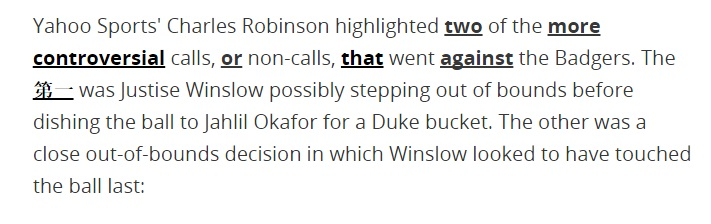
\includegraphics[width=0.45\textwidth]{software_design_2.jpg}
  \caption{Screen shot of Translating Component}
  \label{fig:software_design_2}
\end{figure}
After the original web page, our chrome extension will fetch the content of the news and pass them to the server paragraph by paragraph. After receiving the content, server will compare every word in the paragraph with the words in our vocabulary. If there are some matches, which simply means there are some words that need to be replaced. As every English word might have a few Chinese meanings, our server must select the most appropriate translation among all the meanings. The way that we are trying to solve this problem so far is to compare all the Chinese meanings with the translation of the whole sentence from Bing Translate. If any of the Chinese meanings is the substring of the translation of the sentence, our server will choose that meaning (This is not a proper and accurate way to solve this problem, but it is much better than randomly choose one Chinese meanings. Also, this would be my main research problem that I need to solve next semester). Then, server will pass a JSON string that contains all the words that need to be replaced, their Chinese meanings as well as their pronunciations back to front end. Then, front end will replace the content of the news paragraph by paragraph, in which some words have been replaced. Figure \ref{fig:software_design_2} is the screen shot of this component.
\\
\subsubsection{Learning}
\begin{figure}[ht]
  \centering
    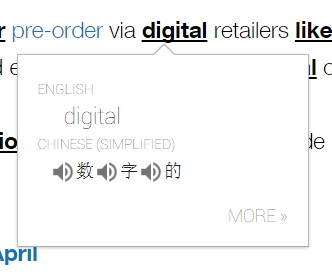
\includegraphics[width=0.3\textwidth]{software_design_4.jpg}
  \caption{Screen shot of popover with highlighted English word}
  \label{fig:software_design_4}
\end{figure}

\begin{figure}[ht]
    \centering
    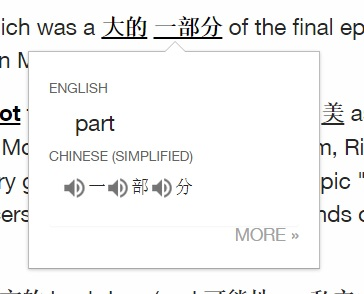
\includegraphics[width=0.3\textwidth]{software_design_5.jpg}
    \caption{Screen shot of popover with highlighted Chinese word}
    \label{fig:software_design_5}
\end{figure}
\\
By moving mouse on the Chinese word for one second, a window with its English meaning and pronunciation will pop over. Figure \ref{fig:software_design_4} is the screen shot of the pop over without its example sentence. If user want to know how to use this word, he can just click the button next to the pronunciation to get the example sentences of this word. After user click the button to get example sentence, our extension will send a request to server and wait for server' response. There is another way of doing this, which is simply get the example sentences together with the words in the Translating component. However, the example sentences contains much more characters comparing with the pronunciation. We want to maximize the loading speed and minimize the data transferred between front end and server, so we decided to split the pop over content into two request. Figure \ref{fig:software_design_5} is the screen shot of the pop over with its example sentences.
\\
\subsubsection{Testing}
\begin{figure}[ht]
\centering
  \centering
  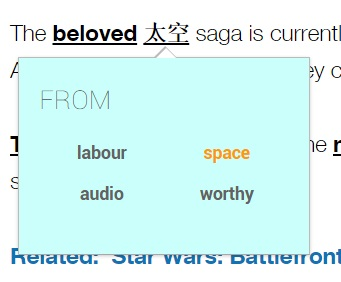
\includegraphics[width=0.3\textwidth]{software_design_7.jpg}
  \caption{Screenshot of English test popover}
  \label{fig:software_design_7}
\end{figure}

\begin{figure}[ht]
    \centering
  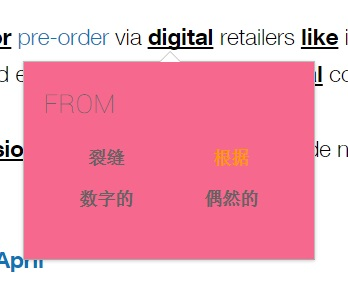
\includegraphics[width=0.3\textwidth]{software_design_8.jpg}
  \caption{Screen shot of Chinese test popover}
  \label{fig:software_design_8}
\end{figure}
When user has encountered the same word for a few times, our system will generate a quiz about this word for him.  If user move mouse over this replaced word, a window with a quiz will pop over. After user select one option, this window will tell user the correct answer and sent whether the answer is correct to server. Figure \ref{fig:software_design_7} is the screen shot of our testing popover in English. Figure \ref{fig:software_design_8} is the screen shot of our testing popover in Chinese.

\section{Distractors Generation Algorithm}
The key research topic here is to investigate a way to automatically generate suitable distractors for a certain vocabulary test. The distractors are generated in English form.
\subsection{Collecting category-related words}
To generate good category-related distractors, it is essential to gather enough words that are more related in a certain category to serve as distractors candidates.
\\
To find good “category-related” words, it is essential to get the words from those already classified news articles. The process involves 3 steps, crawling news contents from popular news website, preprocessing, and classifying word category.
\\
\subsubsection{Crawling news content}
Several web crawlers are designed to get news content from different popular news websites. The crawler will detect URLs from each news website’s main page as and its sub-category pages. For example, there are sub-categories like “football”, “basketball” under main category “Sports”, and the crawler is able to crawl URLs from “football” page and “basketball” page as well. 
\\
After detailed comparison of most news websites, I divided news articles into seven categories, namely “World”, “Technology”, “Sports”, “Entertainment”, “Finance”, “Health” and “Travel”. Most news articles can be classified into one of the seven categories. The web crawler will store all paragraph tags from each websites and store them as one file under one category. 
\\
In this experiment, around 1400 news articles, i.e. 200 news articles from each category are crawled and stored locally. Post natural language processing is then applied to this category corpus.
\\
\subsubsection{Preprocessing}
After storing all the news articles document into each category, the server uses Natural Language Tool Kit \cite{edw09} for word tokenizing and POS Tagging. The system will store the POS tag of each word. After elimination of all non-English words and those words that contain special symbols, like ``O’Real", ``S\$40", all words that contains only alphabetic letters are conserved. All stop words are also eliminated as well. They are stored as lower case for the ease of future process.
\\
\subsubsection{Classification}
In statistical analysis step, the server counts the document frequency of each word in all those stored news articles, i.e. if word “scored” appeared 4 times in one article, it will only be counted as once. By following this approach we can successfully reduce the bias of some words only appear a lot of times in one article while don’t appear often in other article. As we are storing similar number of articles in each category, this approach will provide a fair comparison of each word’s popularity among different categories. After this step we will know the document frequency count of each word in different category. 
Assume C is the list of category names, and f(w, C(i))=m means word w appeared in category C(i) for m times, then the sum weight of word w as sw(w) is calculated in Equation~\ref{equation:Distractor_1}:
\\
\begin{equation}
sw (w) = \sum_{i=1}^{n} f(w,C(i))
\label{equation:Distractor_1}
\end{equation}  
\\
The average weight of word w as aw(w) is calculated in Equation~\ref{equation:Distractor_2}::
\\
\begin{equation}
aw (w) = sw (w)/n 
\label{equation:Distractor_2} 
\end{equation}  
\\
A word w is classified into category C(i) if it satisfies Equation~\ref{equation:Distractor_3}::
\\
\begin{equation}
f (w, C(i)) - aw(w) >= \delta
\label{equation:Distractor_3} 
\end{equation}  
\\
The confidence factor δ can be a positive integer between 0 and the average number of articles in each category. It means on average, the word w must appear in a specific category C(i) δ times more than it appear in other category before it can be classified into category C(i).
\\
In the example below in Figure 18, frequency counts for word “investment” in each category are displayed. It is obvious that sw(“investment”) = 2 + 1 + 2 + 10 + 3 + 2 + 1 = 21, thus aw(“investment”) = sw(“investment”)/7 = 3, in this case if we choose a confidence factor δ=3, word “investment” will be classified into category “Finance”, as 10 – 3 \textgreater δ = 3. However, it we choose a very big δ, for example δ= 8, then word “investment” will not be classified into any category.
\\
\begin{table}[ht]
    \caption{Example of classification word into category}
    \begin{center}
    \begin{tabular}{| p{3.5cm} | p{3cm} |}
        \hline
        Category & Investment\\
        \hline
        Technology & 2 \\
        \hline
        World & 1 \\
        \hline
        Sports & 2 \\
        \hline
        Finance & 10 \\
        \hline
        Entertainment & 3 \\
        \hline
        Health & 2 \\
        \hline
        Travel & 1\\
        \hline
    \end{tabular}
    \end{center}
\end{table}
\\
It is obvious that a higher confidence factor value will result in less number words get classified, but it will result in getting words that are more accurate. A lower confidence factor value will result in more number of words get classified, but less accurate in each category. In this experiment, after several round of tests and analysis, we chose a confidence factor value of 10, which is capable of producing enough number of classified words while maintaining the accuracy.
\subsection{Generating distractors}
My selection strategy in choosing distractors takes following parameters:
\begin{itemize}
\item News website URL
\item News sentence
\item Word to test
\item User’s knowledge level of the word
\end{itemize}
\subsubsection{Detect news category}
After getting the news URL, our system needs to determine the category of the news. Based on the analysis from most popular news URLs, there is a set of common identifiers that can identify the category of the news article. For example, technology news URL often contains “/tech”, “/science”, and if we find these strings in news URL, we will classify this news URL into “Technology” category. The algorithm will go through all category identifier in the list, and will return the category name the moment it finds a match. The current list of category provides reasonable accuracy for the purpose of detecting news category.
\\
\subsubsection{Detect Part-Of-Speech Tag}
Given the target word and the target sentence, it is easy to run the NLTK POS tagger to get the correct POS tag of this word. This step is essential to help select distractors with similar forms, i.e. if the target word is adjective, it will be appropriate to choose three other adjectives, not verbs, as distractors.
\\
\subsubsection{Semantic Distance}
Before we go to explain the next step, it is essential to introduce the semantic distance calculator we used in the server implementation. 
\\
The perspective of semantic relatedness or its inverse, semantic distance, is a concept that indicates the likeness of two words. It is more general than the concept of similarity as stated in WordNet’s synset relation. Similar entities in WordNet are classified into same synset based on their similarity. However, dissimilar entries may also have a close semantic connection by lexical relationships  such as meronymy (car-wheel) and antonymy (hot-cold), or just by any kind of functional relationship or frequent association(pencil-paper, penguin-Antarctica) \cite{ale01}. Semantic distance calculator aims to calculate the semantic relatedness score between two words.
\\
There are many approaches to calculate semantic relatedness score. In this application, we are using Lin Distance \cite{lin98} to calculate the semantic distance between two concepts. The detail of Lin Distance methodology is explained as follows.
\\
Lin attempted to define a measure of semantic similarity that would be both universal and theoretically justified. There are three intuitions that he used as a basis:
\begin{itemize}
\item The similarity between arbitrary objects A and B is related to their commonality; the more commonality they share, the more similar they are;
\item The similarity between A and B is related to the differences between them; the more differences they have, the less similar they are.
\item The maximum similarity between A and B is reached when A and B are identical, no matter how much commonality they share. 
\end{itemize}
\\
Based on the intuition above, Lin proposed his approach in measuring similarity between two concepts c1, c2 in Equation~\ref{equation:Distractor_4}:
\\
\begin{equation}
sim(c1,c2) = \frac{2*log_p(lso(c1,c2))}{log_p(c1)+log_p(c2)}
\label{equation:Distractor_4}
\end{equation}  
\\
where p(c) denotes the probability of encountering concept c, and lso(c1,c2) denotes the lowest common subsumer, which is the lowest node in WordNet hierarchy that is a hypernym of c1 and c2. 
\\
The distance calculator will return a score from 0 to 1, as can be easily seen from the formula above. If the score is closer to 1, it means the two words are closer in semantic sense. This distance calculator will play an important role in the following algorithm. 
\\
\subsubsection{Distractors Selection Algorithm}
Based on the input parameters, at this stage the server has already got the current category of the news article and the correct POS tag of the target word to test. The server is going to generate distractors based on user’s knowledge level of the target word to test.
\\
Knowledge level is 1: This indicates that the user has just learnt this word. The algorithm will randomly select three words from current category’s word list. The reason for using randomization is to avoid the situation that similar distractors are generated every time.
\\
Knowledge level is 2: This indicates that the user has known this word for some times. The algorithm will randomly select two words from the current category’s word list as two distractors. Then the algorithm will randomly select word from the current category’s word list and calculated the semantic distance between the selected word and the target word, once the score is above certain threshold, the selected word will be chose as the third distractor. The selection of threshold value will have a direct effect on the speed of distractors generation process. As a very high threshold value will result in more rounds of calculation in semantic distance calculator, and it will take a long time before the distractors are returned to the front end. After several rounds of analysis of each category’s words and the results returned from semantic distance calculator, the threshold value of 0.1 is selected.
\\
Knowledge level is 3: This indicates that the user has a good understanding of the word already; the algorithm will choose distractors solely based on results returned from semantic distance calculator. Similar to the approach when knowledge level is 2, the algorithm will randomly select word from current category’s word list and calculate the semantic distance between the selected word and the target word. If the score is above certain threshold, the selected word is chosen as one of the distractors. The process is continued until the server can find three distractors. 
\\
\section{Word Sense Disambiguation System}
\begin{CJK}{UTF8}{gbsn}
As we all know, one word may have multiple translations in another language, and our extension is expected to select the most appropriate one based on the context.We call such translation selection as cross-lingual word sense disambiguation (WSD).

In this following, I describe four approaches that I have tried to accomplish WSD system, which is also my main progress in the second semester. The four approaches are: 

\begin{itemize}
\item Frequency based: always selecting the most frequent translation (the baseline),
\item Part-of-Speech Tag based: selecting the translation based on the Part-of-Speech Tag of the English word
\item Translation based: Selecting the translation based on the result from existing Machine Translation systems
\item Category based: Selecting the translation based on the category of the news article
\end{itemize}

\begin{table*}[t]
  \caption{Example input/output of WSD}
  \label{table:wsd_1}
  \begin{center}
  \begin{tabular}{| p{3cm} | p{1cm} | p{3.5cm} | p{1.2cm} | p{1.3cm}| p{0.8cm} | p{0.9cm} | p{1cm} |}
    \hline
    English Sentence & Word & Dictionary & Baseline & Category & Bing & Bing+ & Bing++ \\
    \hline
    ... treating me like family ... & like & \parbox[t]{3cm}{verb : 喜欢, 爱...\\ ... \\preposition : 好像, 好比 ...} & 喜欢 & 好像 & & & \\
    \hline
    ... painting a picture of urban street life ... & picture & \parbox[t]{3cm}{... 相, 影, 影片(entertainment), 帧, 想象, 画 ...} & & 影片 & & & \\
    \hline
    ... pistol a pump shotgun ... & pump & \parbox[t]{3cm}{verb:抽, 抽水, 打气, 唧, 唧筒, 套\\ noun:抽水机, 唧筒} & & & 唧筒 & & \\
    \hline
    ... have made it into the worlds top 40 clubs ... & top & \parbox[t]{3cm}{顶部, 顶端, 顶, 颠, 盖, 极 ...} & 顶部 &  & 顶 & 顶级 & \\
    \hline
    state department spokeswoman ... & state & \parbox[t]{3cm}{...陈, 陈说, 称, 称述, 发表, 发言...} & & & 发言 & 发言人 & 国家 \\
    \hline
    ...  ... &  & \parbox[t]{3cm}{...  ...} & & & & & \\
    \hline
  \end{tabular}
  \end{center}
\end{table*}

\subsection{Baseline}
The simplest way to select a translation from the candidates is by random. However, the correctness of this method is very low, probably less than 20\%, and is not a good baseline for other methods to compete with. Another simple idea is to always select the most commonly used translation. Luckily, when I crawled the dictionary, Google Translate does provide usage frequency of each Chinese Translation.  This turns out to be a much better result, and thus serves as a fair baseline method.

\subsection{Part-of-Speech Tagger}
As we all know, many English words have more than one Part-of-Speech (POS) tags and their Chinese translations in different POS may differ a lot. For example, the word ``book" has two POS tags, noun and verb. If it is used as a noun, mostly it means a handwritten or printed work of fiction or nonfiction, which should be translated as \begin{CJK}{UTF8}{gbsn}``书"\end{CJK}, and mostly means to reserve if used as a verb, which should be translated as \begin{CJK}{UTF8}{gbsn}``预定"\end{CJK}. Therefore, getting the POS tag of the English word might help us identify its sense or the Chinese translation. We decide use Stanford Log-linear Part-of-Speech Tagger \cite{Toutanova2003}.

Firstly, if the word "like" need to be translated, the algorithm will fetch all the Chinese translations as well as their Part-of-Speech tag from our dictionary. Secondly, the algorithm will send the original English sentence to Part-of-Speech Tagger, which is a Java package and has been wrapped into a server. After the client has got the output from the server, it will fetch the corresponding tag and match it to Part-of-Speech tag based on the guidelines mentioned above. Lastly, it will select the translations based on the POS.

\subsection{News Category}
The word ``interest" have two very different translations when it is used as a noun. One translation is about ``the feeling of a person whose attention, concern, or curiosity is particularly engaged by something", which should be translated as ``兴趣". The other translation is about ``a share, right, or title in the ownership of property", which should be translated as ``利息". It is quite obvious that the second sense is mostly used in financial related topics. Therefore, analysing the category of the original article and selecting the translation with the same category label might help disambiguate the word meaning.

In Table~\ref{table:wsd_1}, word ``picture" is the word that need to be translated. Firstly, the algorithm will fetch all the Chinese translations for word ``picture" and only the word ``影片" has a category ``entertainment". Next, the algorithm will fetch the category of the English news article from the URL, which is also ``entertainment".In this case, the algorithm will use ``影片" as the translation for word ``picture". If a few words shares the same category, the algorithm will choose the translation with the highest frequency of use.

\subsection{Machine Translation}
Since our target is to select the most appropriate translation based on the context, using existing Machine Translation (MT) systems is also a good approach, as all of them will certainly translate words based on the context. After I tried a few on-line or off-line MT systems, We decide to use Bing Translator as our Machine Translation system.

\subsubsection{Bing}

In the example, the original English sentence is ``including a 45-caliber pistol a pump shotgun and an ar-15 rifle" and ``pump" is the word that we want to translate. Firstly, this algorithm will fetch all the Chinese translations from the database. Next, it will send the original English sentence to Bing Translator using the API provided by Microsoft and get the result that returned from Bing Translator. After that, for each Chinese translation, I will check whether this translation is a substring of the Bing Translator result. If there are a few translations that can match with the Bing Translator result, I will select the longest translation. If there are a few translations with the same length and all of them can match with the Bing Translator result, I will select the translation with the highest frequency of use. In this example, both ``唧" and ``唧筒" are the substrings of Bing Translator result. As ``唧筒" have two characters and ``唧" only have one character, this algorithm will take ``唧筒" as the final result.

\subsubsection{Bing+}
 is the approach of using Bing Translator together with Stanford Word Segmenter, and I would like to use Bing+ to represent this algorithm. Step one, two and three has been described in the previous section as it is exactly the same as Bing approach. From Bing approach, this algorithm will generate ``顶" as the result. After that, Bing+ approach will send the Chinese sentence returned from Bing Translator to Stanford Word Segmenter. Then, this algorithm will use the segmented word that contains the Bing result as a substring or equals to the Bing result as the final result. In this example, the final result of Bing+ is ``顶级" which is the best result that can be generated from the result of Bing Translator and also a result that does not covered by our dictionary.

\subsubsection{Bing++}
The Bing++ algorithm is basically the approach of using Bing+ approach together with the Microsoft Bing Word Alignment. First few steps are exactly the same as Bing+ approach. In this example, ``state" is the word that need to be translated. The result from Bing+ approach is ``发言人", which is the translation of ``spokeswoman", because the Chinese translation ``发言" can be translated from both ``state" and ``spokeswoman". Then step five will send the original English sentence to Bing Word Alignment. Now, there will be two final results, one from Bing+ approach and the other one from Bing Word Alignment and the algorithm will choose the correct one from these two results. In this example, ``state" will match with ``国家" and the algorithm will choose ``国家" as the final result as well.

\subsection{WSD System}
Our Word Sense Disambiguate System can be evaluated from two important aspects: coverage (i.e., is able to return a translation) and accuracy (i.e., the translation is proper). To this end, I manually annotate the ground truth.

\begin{table}[ht]
  \caption{Coverage for different approaches}
  \label{table:evaluation_1}
  \begin{tabular}{| p{2cm} | p{2cm} | p{2cm} |}
    \hline
     & Coverage & Accuracy\\
    \hline
    Baseline & 100\% & 57.3\%\\
    \hline
    POSTagger & 94.5\% & 55.2\%\\
    \hline
    News Category & 2.0\% & 7.1\%\\
    \hline
    Bing & 78.5\% & 79.8\%\\
    \hline
    Bing+ & 75.7\% & 80.9\%\\
    \hline
    Bing++ & 76.9\% & 97.4\%\\
    \hline
  \end{tabular}
\end{table}

Table~\ref{table:evaluation_1} column two contains the coverage for different approaches. As the algorithm will try to translate some word only if it is covered by our dictionary, the coverage for Baseline is always 100\%. The coverage for Bing, Bing+, Bing++ and POSTagger are roughly the same and all of them are acceptable. However, the coverage for News Category approach is only 2.0\%. One reason is that when I set the threshold for assigning categories for Chinese word, I purposely make it very high to maximize the accuracy. If the accuracy is quite high, which means this approach is quite useful, then I will lower the threshold and find the balance point.

Figure~\ref{table:evaluation_1} column three contains the accuracy of all the approaches. The last column is the accuracy for News Category approach and it is only 7.1\%. As mentioned in above Chapter, since the accuracy is very low, there is no need to lower the threshold and try to allocate more categories for Chinese words. The accuracy for Baseline is 57.3\%, which is already a fairly hight accuracy. The accuracy for  POSTagger is around 55.2\% also, which is a bit lower than our expectation. The accuracy for Bing++ is 97.4\% which I think is a very good result and it is already very hard to improve. Therefore, based on my test results, Bing++ is the best approach among these five approaches.

\end{CJK}
\section{Results}
This project has two main parts, Chrome Extension and WSD system. The Chrome Extension part is a  software development project and the best way to evaluate is to listen to users' voice. The WSD system is a standard research problem and can be evaluated with ground-truth, reporting its performance
%tested from a few very standard aspects, 
by coverage and accuracy.
\subsection{Chrome Extension}
There are a few standard aspects that can be evaluated from the Chrome Extension part, such as User Interface (UI) design, loading speed and the functionality. UI design and functionality are more related to front end, while the loading speed is highly correlated to the back end. As this project is a joint work, and I am responsible  for the front end, I limit my focus to evaluate the UI design and functionality by surveying users.
Also, as mentioned in the above chapters, we did a user requirement survey before we really start this project. From this survey, we roughly know  our potential customers' expectation and we need to check whether our Chrome Extension could satisfy them. I got 16 different responses, 15 of them are between 18 and 24, and 11 of them are professional in Chinese.
\\
For the details of the survey questions and survey results, please refer to the Appendix. In this survey, I made some screen shots of our Chrome Extension and ask subjects about their opinions. 
Most of them think that replacing some words with their corresponding Chinese translation will not influence their normal reading, but they will feel a bit uncomfortable and prefer to read the original English articles. Based on their voice, I decide to highlight the original English words as default setting instead of replacing the English words with their Chinese Translations. Besides, most subjects think our Chrome Extension is nice and would like to try it when they are going to learn a new language.
\\
\subsection{WSD System}
% Tao: 1. Why you change eval dataset?  This makes your evaluation results less convicing. I tried my best to address it. But you need to fix this problem in workshop paper. 2. You need to report the exact size of your eval dataset, e.g., # of sentences/words.
Our Word Sense Disambiguate System can be evaluated from two important aspects: coverage (i.e., is able to return a translation) and accuracy (i.e., the translation is proper). To this end, I manually annotate the ground truth. Each approach was evaluated  right after I had implemented it, therefore,  they was tested against a random but different set of recent news articles from CNN.  Though the evaluation datasets are different, it is still fair to compare their results, as the size of all dataset is sufficiently large. 


Firstly, we want our algorithm to return at least one result instead of blank. For POSTagger approach, if our dictionary do not cover the Part-of-Speech generated from Stanford POSTagger, the algorithm will return nothing. For News Category approach, as the algorithm will only assign categories for some of the Chinese translations and not all Chinese news categories can match with a English news category, so the algorithm sometimes will return nothing as well. For Bing+ and Bing++ approach, if none of the Chinese translations is the substring of the Bing result, the algorithm will return nothing. For Bing++ approach, if the word alignment information is phrase to phrase matching, for example, it may give a matching between ``in order to" and its Chinese translation, the algorithm will return nothing. Alternatively, for all the listed algorithm listed above, they can always return the translation with the highest frequency of use, but in this case, we cannot know whether the result is generated from the algorithm itself or just the baseline. That's why I choose to return a blank instead of the translation with the highest frequency of use.

\begin{table}[ht]
  \caption{Coverage for different approaches}
  \label{table:evaluation_1}
  \begin{tabular}{| p{2cm} | p{2cm} | p{2cm} |}
    \hline
     & Cover & Coverage\\
    \hline
    Baseline & 707/707 & 100\%\\
    \hline
    POSTagger & 668/707 & 94.5\%\\
    \hline
    News Category & 14/707 & 2.0\%\\
    \hline
    Bing & 555/707 & 78.5\%\\
    \hline
    Bing+ & 535/707 & 75.7\%\\
    \hline
    Bing++ & 544/707 & 76.9\%\\
    \hline
  \end{tabular}
\end{table}

Table~\ref{table:evaluation_1} contains the coverage for different approaches. As the algorithm will try to translate some word only if it is covered by our dictionary, the coverage for Baseline is always 100\%. The coverage for Bing, Bing+, Bing++ and POSTagger are roughly the same and all of them are acceptable. However, the coverage for News Category approach is only 1.9\%. One reason is that when I set the threshold for assigning categories for Chinese word, I purposely make it very high to maximize the accuracy. If the accuracy is quite high, which means this approach is quite useful, then I will lower the threshold and find the balance point.
\\
Secondly, we want our algorithm to be as accurate as possible, and the most ideal situation is that all the translation returned from the algorithm is the correct or the most appropriate translation in that context. When I evaluate the accuracy of these few approaches, I use a few news articles from CNN as the input data and manually select the most appropriate translation for all the output data. After that, I will compare the result from the algorithm and the result that I manually generated and get the accuracy.
\\
\begin{table}[ht]
  \caption{Accuracy for different approaches}
  \label{table:evaluation_3}
  \begin{tabular}{| p{2cm} | p{2cm} | p{2cm} |}
    \hline
     & Correct & Accuracy\\
    \hline
    Baseline & 405/707 & 57.3\%\\
    \hline
    POSTagger & 369/668 & 55.2\%\\
    \hline
    News Category & 1/14 & 7.1\%\\
    \hline
    Bing & 443/555 & 79.8\%\\
    \hline
    Bing+ & 433/535 & 80.9\%\\
    \hline
    Bing++ & 534/544 & 98.2\%\\
    \hline
  \end{tabular}
\end{table}
\\
Figure~\ref{table:evaluation_3} contains the accuracy of all the approaches. The last column is the accuracy for News Category approach and it is only 30\%. As mentioned in above Chapter, since the accuracy is very low, there is no need to lower the threshold and try to allocate more categories for Chinese words. The accuracy for Baseline is 69\%, which is already a fairly hight accuracy. The accuracy for Bing and POSTagger is around 69\% also, which is a bit lower than our expectation. The accuracy for Bing++ is 97\% which I think is a very good result and it is already very hard to improve. Therefore, based on my test results, Bing++ is the best approach among these five approaches.
\\
\input{6_Application}

% include your own bib file like this:
%\bibliographystyle{acl}
%\bibliography{acl2015}
% use socreport.bst
\bibliographystyle{acl}
\bibliography{acl2015}

\end{document}
\clearpage\end{CJK*}